\documentclass{article}
\usepackage{graphicx}
\usepackage{amsmath}
\usepackage{tikz}
\usetikzlibrary{calc,angles,positioning,intersections,quotes,decorations.markings}
\usepackage{listings}
\usepackage{xcolor}
\lstset{
    frame=tb,
    tabsize=4,
    showstringspaces=false,
    numbers=left,
    commentstyle=\color{gray},
    keywordstyle=\color{blue},
    stringstyle=\color{red}
}

\begin{document}

	\title{Distance from a quadrilateral to a point}
	\author{Benjamin Loison}
	\date{22 decembre 2018}
	\maketitle

	\tableofcontents
	\clearpage

	\section{Opening speech}

		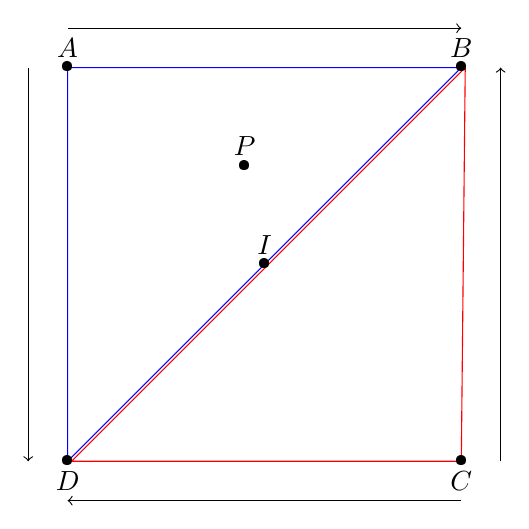
\begin{tikzpicture}

			\coordinate (A) at (0, 5);
			\coordinate (B) at (5, 5);
			\coordinate (C) at (5, 0);
			\coordinate (D) at (0, 0);
			\coordinate (I) at (2.5, 2.5);
			\coordinate (P) at (2.25, 3.75);

			\draw[blue] (A) -- (B) -- (D) -- (A);
			\draw[red] (5.05, 5) -- (C) -- (0.05, 0) -- (5.05, 5);

			\foreach \Point in {(A), (B), (C), (D), (I), (P)}
			{
					\node at \Point {\textbullet};
			}

			\node at ($(A)! 2.5mm! (A)$){$A$};
			\node at ($(B)! 2.5mm! (B)$){$B$};
			\node at ($(C)! -2.5mm! (C)$){$C$};
			\node at ($(D)! -2.5mm! (D)$){$D$};
			\node at ($(I)! 2.5mm! (I)$){$I$};
			\node at ($(P)! 2.5mm! (P)$){$P$};

			\draw [->] (0, 5.5) -- (5, 5.5);
			\draw [->] (-0.5, 5) -- (-0.5, 0);
			\draw [->] (5, -0.5) -- (0, -0.5);
			\draw [->] (5.5, 0) -- (5.5, 5);

		\end{tikzpicture}\\\\

		% \begin{figure}
		%		\centering
		%		\includegraphics[scale=0.3]{quadrilateral.jpg}
		% 	\caption{Vertical view}
		% 	\label{fig1}
		% \end{figure}
		
		We work with four points $A$, $B$, $C$, $D$ and $P$ which we know the components (x, y, z).\\
		And we will have a lot of work on $P$ which is the point where is the player.\\
		The aim of these algorithms is to compute the distance between the player and the ground under him.
		%The aim of these algorithms is to compute the distance between the player and the nearest point of the ground.\\
		To solve this issue we are going to slice the quadrilateral in two, in order to get two triangles: $ABD$ and $BCD$.\\
		Likewise we have one point and two vectors for each triangle, so we can define a unique plane.

	\section{Computing of a normal vector to a triangle}

		Let's first work on the $ABD$ triangle, the $BCD$ will have quite a same process.\\
		We have:\\
		$A, B, C(x_K, y_K, z_K)$\\
		And more especially:\\\\
		
		$A(x_A, y_A, z_A)$\\
		$\left\{\begin{array}{r c l}
			\overrightarrow{AB}=(x_B - x_A, y_B - y_A, z_B - z_A)\\
			\overrightarrow{AD}=(x_D - x_A, y_D - y_A, z_D - z_A)
		\end{array}\right.$\\\\

		Let's set $\vec{n}$ a normal vector: $(\vec{n}_x, \vec{n}_y, \vec{n}_z)$\\
		We have:\\\\
		
		$\left\{\begin{array}{r c l}
			\overrightarrow{AB}.\vec{n} = 0\\
			\overrightarrow{AD}.\vec{n} = 0
		\end{array}\right.$\\\\
		
		Notice: $\vec{a}.\vec{b}=\vec{a}_x * \vec{b}_x + \vec{a}_y * \vec{b}_y + \vec{a}_z * \vec{b}_z$\\
		
		Which is equivalent to:\\\\
		
		$\left\{\begin{array}{r c l}
			\overrightarrow{AB}_x * \vec{n}_x + \overrightarrow{AB}_y * \vec{n}_y + \overrightarrow{AB}_z * \vec{n}_z = 0\\
			\overrightarrow{AD}_x * \vec{n}_x + \overrightarrow{AD}_y * \vec{n}_y + \overrightarrow{AD}_z * \vec{n}_z = 0
		\end{array}\right.$\\\\
		
		So two equations for three unknows, this is normal because we will fix one of this unknown (it will correspond as something like fixing the length of $\vec{n}$).\\
		This indeed depends on $\vec{n}_z$, which will be fixed to 1 (and not 0 to escape $\vec{0}$) and it simplify a final calculus.\\\\
		
		$\left\{\begin{array}{r c l}
			\overrightarrow{AB}_x * \vec{n}_x + \overrightarrow{AB}_y * \vec{n}_y + \overrightarrow{AB}_z = 0\\
			\overrightarrow{AD}_x * \vec{n}_x + \overrightarrow{AD}_y * \vec{n}_y + \overrightarrow{AD}_z = 0
		\end{array}\right.$\\\\
		
		\subsection{First method with substitution}
		
			\textcolor[rgb]{1,0,0}{Important: this method here doesn't take care about hypothesis on denominator so please switch to Cramer's method}\\\\
		
			So:\\\\
			
			$\left\{\begin{array}{r c l}
				\vec{n}_x = - \frac{\overrightarrow{AB}_y * \vec{n}_y + \overrightarrow{AB}_z}{\overrightarrow{AB}_x}\\
				\vec{n}_y = - \frac{\overrightarrow{AD}_x * \vec{n}_x + \overrightarrow{AD}_z}{\overrightarrow{AD}_y}
			\end{array}\right.$\\\\
			
			Finally:\\\\
			
			$\vec{n}_x = \frac{1}{\overrightarrow{AB}_x} * \left(\frac{\overrightarrow{AB}_y * (\overrightarrow{AD}_x * \vec{n}_x + \overrightarrow{AD}_z)}{\overrightarrow{AD}_y} - \overrightarrow{AB}_z\right)$\\\\
			
			Or:\\\\
			
			$\vec{n}_x = \frac{1}{\overrightarrow{AB}_x}\left(\frac{\overrightarrow{AB}_y * \overrightarrow{AD}_z}{\overrightarrow{AD}_y} - \overrightarrow{AB}_z\right) + \frac{\overrightarrow{AB}_y * \overrightarrow{AD}_x * \vec{n}_x}{\overrightarrow{AB}_x * \overrightarrow{AD}_y}$\\\\
			
			So:\\\\
			
			$\vec{n}_x - \frac{\overrightarrow{AB}_y * \overrightarrow{AD}_x * \vec{n}_x}{\overrightarrow{AB}_x * \overrightarrow{AD}_y} = \frac{1}{\overrightarrow{AB}_x}\left(\frac{\overrightarrow{AB}_y * \overrightarrow{AD}_z}{\overrightarrow{AD}_y} - \overrightarrow{AB}_z\right)$\\\\
			
			$\vec{n}_x * \left(1 - \frac{\overrightarrow{AB}_y * \overrightarrow{AD}_x}{\overrightarrow{AB}_x * \overrightarrow{AD}_y}\right) = \frac{1}{\overrightarrow{AB}_x}\left(\frac{\overrightarrow{AB}_y * \overrightarrow{AD}_z}{\overrightarrow{AD}_y} - \overrightarrow{AB}_z\right)$\\\\
			
			$\vec{n}_x * \left(\frac{\overrightarrow{AB}_x * \overrightarrow{AD}_y - \overrightarrow{AB}_y * \overrightarrow{AD}_x}{\overrightarrow{AB}_x * \overrightarrow{AD}_y}\right) = \frac{1}{\overrightarrow{AB}_x}\left(\frac{\overrightarrow{AB}_y * \overrightarrow{AD}_z}{\overrightarrow{AD}_y} - \overrightarrow{AB}_z\right)$\\\\
			
			$\vec{n}_x = \frac{\overrightarrow{AB}_x * \overrightarrow{AD}_y}{(\overrightarrow{AB}_x * \overrightarrow{AD}_y - \overrightarrow{AB}_y * \overrightarrow{AD}_x) * \overrightarrow{AB}_x}\left(\frac{\overrightarrow{AB}_y * \overrightarrow{AD}_z}{\overrightarrow{AD}_y} - \overrightarrow{AB}_z\right)$\\\\

			$\vec{n}_x = \frac{\overrightarrow{AD}_y}{\overrightarrow{AB}_x * \overrightarrow{AD}_y - \overrightarrow{AB}_y * \overrightarrow{AD}_x}\left(\frac{\overrightarrow{AB}_y * \overrightarrow{AD}_z}{\overrightarrow{AD}_y} - \overrightarrow{AB}_z\right)$\\\\
			
			As a result, we have:\\\\
			
			$\vec{n}_x = \frac{\overrightarrow{AB}_y * \overrightarrow{AD}_z - \overrightarrow{AD}_y * \overrightarrow{AB}_z}{\overrightarrow{AB}_x * \overrightarrow{AD}_y - \overrightarrow{AB}_y * \overrightarrow{AD}_x}$\\\\
			
			To sum up:\\\\
			
			$\vec{n}\left(\frac{\overrightarrow{AB}_y * \overrightarrow{AD}_z - \overrightarrow{AD}_y * \overrightarrow{AB}_z}{\overrightarrow{AB}_x * \overrightarrow{AD}_y - \overrightarrow{AB}_y * \overrightarrow{AD}_x}, - \frac{\overrightarrow{AD}_x * \vec{n}_x + \overrightarrow{AD}_z}{\overrightarrow{AD}_y}, 1\right)$\\\\
			
			Or, if we assume that: $\vec{n}_y = - \frac{\overrightarrow{AD}_x * \vec{n}_x + \overrightarrow{AD}_z}{\overrightarrow{AD}_y}$\\\\
			
			$\vec{n}\left(- \frac{\overrightarrow{AB}_y * \vec{n}_y + \overrightarrow{AB}_z * \vec{n}_z}{\overrightarrow{AB}_x}, \vec{n}_y, 1\right)$\\\\
			
			Notice: for the algorithm part, it is important to remind us that for optimization, we need to firstly compute $\vec{n}_x$ before $\vec{n}_y$ (to use it to compute $\vec{n}_y$ of course).\\
			
			\begin{lstlisting}[language=C++, caption={Here is the implementation in C++ to compute $\vec{n}$}]
Vector3D normalVectorOfTriangle(Vector3D AB, Vector3D AD)
{
	double Nx = (AB.y * AD.z - AD.y * AB.z) / (AB.x * AD.y - AB.y * AD.x);
	double Ny = -(AD.x * Nx + AD.z) / AD.y;
	return Vector3D(Nx, Ny, 1);
}
		\end{lstlisting}
		
		\subsection{Second method with Cramer's determinant}
	
			Slackness... (hope the first method works)\\
			Let's write a few lines to check several things:\\
			We got:\\\\
			
			$\left\{\begin{array}{r c l}
				\overrightarrow{AB}_x * \vec{n}_x + \overrightarrow{AB}_y * \vec{n}_y = - \overrightarrow{AB}_z\\
				\overrightarrow{AD}_x * \vec{n}_x + \overrightarrow{AD}_y * \vec{n}_y = - \overrightarrow{AD}_z
			\end{array}\right.$\\\\
			
			Let's compute the determinant of this system:\\\\
			
			$\Delta = \overrightarrow{AB}_x * \overrightarrow{AD}_y - \overrightarrow{AB}_y * \overrightarrow{AD}_x$\\\\
			
			$\Delta = 0$ if, and only if $\overrightarrow{AB}_x * \overrightarrow{AD}_y - \overrightarrow{AB}_y * \overrightarrow{AD}_x = 0$ if, and only if $\overrightarrow{AB}_x * \overrightarrow{AD}_y = \overrightarrow{AB}_y * \overrightarrow{AD}_x$. If so there is an infinity of solution or there is no solution (depends respectively for a graphical interpretation, if lines are superimposed or not).\\
			If there is no solution, this is the end and if there is an infinity it seems impossible because it means that for two random direction, we will go up of 1.\\\\
			
			Let's assume $\Delta \neq 0$, the pair solution is:\\\\
			
			$\left\{\begin{array}{r c l}
				\vec{n}_x = \frac{\begin{vmatrix}
					 - \overrightarrow{AB}_z & \overrightarrow{AB}_y \\
					 - \overrightarrow{AD}_z & \overrightarrow{AD}_y
				\end{vmatrix}}{\Delta}\\\\
				\vec{n}_y = \frac{\begin{vmatrix}
					 \overrightarrow{AB}_x & - \overrightarrow{AB}_z \\
					 \overrightarrow{AD}_x & - \overrightarrow{AD}_z
				\end{vmatrix}}{\Delta}
			\end{array}\right.$\\\\
			
			Which is equivalent to:\\\\
			
			$\left\{\begin{array}{r c l}
				\vec{n}_x = \frac{\overrightarrow{AB}_y * \overrightarrow{AD}_z - \overrightarrow{AB}_z * \overrightarrow{AD}_y}{\Delta}\\\\
				\vec{n}_y = \frac{\overrightarrow{AB}_z * \overrightarrow{AD}_x - \overrightarrow{AB}_x * \overrightarrow{AD}_z}{\Delta}
			\end{array}\right.$\\\\
			
			Finally:\\\\
			
			$\left\{\begin{array}{r c l}
				\vec{n}_x = \frac{\overrightarrow{AB}_y * \overrightarrow{AD}_z - \overrightarrow{AB}_z * \overrightarrow{AD}_y}{\overrightarrow{AB}_x * \overrightarrow{AD}_y - \overrightarrow{AB}_y * \overrightarrow{AD}_x}\\\\
				\vec{n}_y = \frac{\overrightarrow{AB}_z * \overrightarrow{AD}_x - \overrightarrow{AB}_x * \overrightarrow{AD}_z}{\overrightarrow{AB}_x * \overrightarrow{AD}_y - \overrightarrow{AB}_y * \overrightarrow{AD}_x}
			\end{array}\right.$\\\\
			
			\begin{lstlisting}[language=C++, caption={Here is the implementation in C++ to compute $\vec{n}$}]
Vector3D normalVectorOfTriangle(Vector3D AB, Vector3D AD)
{
	double determinant = AB.x * AD.y - AB.y * AD.x;
	if(determinant == 0)
	{
		cout << "A fatal error occured, map theory involves this impossibility
		(AB, AD): " << AB.x << " " << AB.y << " " << AB.z << " " << AD.x << " "
		<< AD.y << " " << AD.z << endl;
		exit(2);
	}
	double Nx = (AB.y * AD.z - AB.z * AD.y) / determinant;
	double Ny = (AB.z * AD.x - AB.x * AD.z) / determinant;
	return Vector3D(Nx, Ny, 1);
}
			\end{lstlisting}

	\section{Computing the altitude of the ground at the player coordinates}
	
		\subsection{First method}
	
			\textcolor[rgb]{1,0,0}{Reminder: Important: this method here doesn't take care about hypothesis on denominator so please switch to Cramer's method}\\\\
		
			With the previous writing, we got the cartesian equation of a triangle plane:\\\\
			
			$\vec{n}_x * x + \vec{n}_y * y + z + D = 0$ with $D$ a real constant\\\\
			
			Or:\\\\
			
			$D = - \vec{n}_x * x - \vec{n}_y * y - z$\\\\
			
			We compute D with a point of the triangle, for instance: $A$\\\\
			
			$D = - \vec{n}_x * x_A - \vec{n}_y * y_A - z_A$\\\\
			
			Likewise the equation is:\\\\
			
			$\vec{n}_x * x + \vec{n}_y * y + z - \vec{n}_x * x_A - \vec{n}_y * y_A - z_A = 0$\\\\
			
			And we get for the altitude:\\\\
			
			$z = - \vec{n}_x * x - \vec{n}_y * y + \vec{n}_x * x_A + \vec{n}_y * y_A + z_A$\\\\

			\begin{lstlisting}[language=C++, caption={Here is the implementation in C++ to compute the player altitude}]
class Vector3D
{
    public:
        double x, y, z;
        Vector3D(double x, double y, double z);
};

Vector3D::Vector3D(double x, double y, double z) : x(x), y(y), z(z) {}

/*A and P are here considered as points
and we don't need the third component for P*/
double groundAltitude(Vector3D A, Vector3D AB, Vector3D AD, Vector3D P)
{
	double Nx = (AB.y * AD.z - AD.y * AB.z) / (AB.x * AD.y - AB.y * AD.x);
	double Ny = -(AD.x * Nx + AD.z) / AD.y;
    double D = Nx * A.x + Ny * A.y + A.z;
	double altitude = - Nx * P.x - Ny * P.y + D;
	return altitude;
}

double groundAltitudePoints(Vector3D A, Vector3D B, Vector3D C, Vector3D P)
{
    Vector3D AB = Vector3D(B.x - A.x, B.y - A.y, B.z - A.z);
    Vector3D AD = Vector3D(C.x - A.x, C.y - A.y, C.z - A.z);
	return groundAltitude(A, AB, AD, P);
}

int main(int argc, char** argv)
{
    Vector3D A = Vector3D(0, 0, 0);
    Vector3D B = Vector3D(1, 0, 1);
    Vector3D D = Vector3D(0, 1, 1);
    Vector3D P = Vector3D(0.4, 0.25, -99); // the last component doesn't matter

    cout << groundAltitudePoints(A, B, D, P) << endl;
    while(true);
    return 0;
}
			\end{lstlisting}
			
			There is still one kind of problems: division by zero.\\
			It happends if (or):\\\\
			$\left\{\begin{array}{r c l}
					\overrightarrow{AD}_y = 0\\
					\overrightarrow{AB}_x * \overrightarrow{AD}_y - \overrightarrow{AB}_y * \overrightarrow{AD}_x = 0
				\end{array}\right.$\\\\
				
			Which is equivalent to:\\\\
					
			$\left\{\begin{array}{r c l}
					\overrightarrow{AD}_y = 0\\
					\overrightarrow{AB}_x * \overrightarrow{AD}_y = \overrightarrow{AB}_y * \overrightarrow{AD}_x
				\end{array}\right.$\\\\
				
			If $\overrightarrow{AD}_y = 0$ then $\overrightarrow{AB}_y * \overrightarrow{AD}_x = 0$ which means $\overrightarrow{AB}_y = 0$ or $\overrightarrow{AD}_x = 0$\\\\
			
			Condition on the denominator has been forgotten...
			%If $\overrightarrow{AB}_x * \overrightarrow{AD}_y = \overrightarrow{AB}_y * \overrightarrow{AD}_x$ then 
			
		\subsection{Second method}
		
		\begin{lstlisting}[language=C++, caption={Here is the implementation in C++ to compute the player altitude}]
class Vector3D
{
    public:
        double x, y, z;
        Vector3D(double x, double y, double z);
};

Vector3D::Vector3D(double x, double y, double z) : x(x), y(y), z(z) {}

/*A and P are here considered as points
and we don't need the third component for P*/
double groundAltitude(Vector3D A, Vector3D AB, Vector3D AD, Vector3D P)
{
	double determinant = AB.x * AD.y - AB.y * AD.x;
	if(determinant == 0)
	{
		cout << "A fatal error occured, map theory involves this impossibility
		(AB, AD): " << AB.x << " " << AB.y << " " << AB.z << " " << AD.x << " "
		<< AD.y << " " << AD.z << endl;
		exit(2);
	}
	double Nx = (AB.y * AD.z - AB.z * AD.y) / determinant;
	double Ny = (AB.z * AD.x - AB.x * AD.z) / determinant;
    double D = Nx * A.x + Ny * A.y + A.z;
	double altitude = - Nx * P.x - Ny * P.y + D;
	return altitude;
}

double groundAltitudePoints(Vector3D A, Vector3D B, Vector3D C, Vector3D P)
{
    Vector3D AB = Vector3D(B.x - A.x, B.y - A.y, B.z - A.z);
    Vector3D AD = Vector3D(C.x - A.x, C.y - A.y, C.z - A.z);
	return groundAltitude(A, AB, AD, P);
}

int main(int argc, char** argv)
{
    Vector3D A = Vector3D(0, 0, 0);
    Vector3D B = Vector3D(1, 0, 1);
    Vector3D D = Vector3D(0, 1, 1);
    Vector3D P = Vector3D(0.5, 0.5, -99); // the last component doesn't matter

    cout << groundAltitudePoints(A, B, D, P) << endl;
    while(true);
    return 0;
}
		\end{lstlisting}
	
\end{document}